%
%===================================================================================================
%
\documentclass[11pt,aspectratio=169,professionalfonts]{beamer}
%
%===================================================================================================
%
%
%===================================================================================================
%
% Main Modular Preamble Loader
%
%===================================================================================================

%
%===================================================================================================
%
% Packages
%
%===================================================================================================

\usepackage[absolute,overlay]{textpos}

\usepackage[utf8]{inputenc}
\usepackage[T1]{fontenc}

\usepackage{amsmath}
\usepackage{amsfonts}
\usepackage{amssymb}
% the following order matter!!!
\usepackage{lmodern}
\usepackage{bm}

\usepackage{array}
\usepackage{booktabs}
\usepackage{colortbl}
\usepackage{multirow}

\usepackage{graphicx}
\usepackage{tikz}
\usepackage{pgfplots}

\usepackage{framed}
\usepackage{empheq}

\usepackage{xcolor}
\usepackage{soul}

\usepackage{hyperref}
\usepackage{pgfpages}

%\usepackage{minted}

\usepackage[most]{tcolorbox}
\tcbuselibrary{listings}

\pgfplotsset{compat=1.14}
%
%===================================================================================================
%
% TikZ Libraries
%
%===================================================================================================

\usetikzlibrary{
    arrows.meta,
    positioning,
    fit,
    calc,
    shapes.geometric,
    backgrounds,
    matrix
}

% ── Reusable TikZ styles ─────────────────────────────────────
\tikzset{
  block/.style   = {draw, rounded corners, minimum width=2.0cm,
                    minimum height=0.60cm, align=center, font=\small},
  sblock/.style  = {draw, rounded corners, minimum width=1.4cm,
                    minimum height=0.55cm, align=center, font=\small},
  token/.style   = {draw, rounded corners, minimum width=1.1cm,
                    minimum height=0.55cm, font=\small},
  arr/.style     = {->, thick, boIndigo},
  arrg/.style    = {->, gray!60, line width=0.7pt}
}

%
%===================================================================================================
%
% Custom Colors
%
%===================================================================================================

% General accents
\definecolor{accent}{RGB}{200,60,50}
\definecolor{Accent}{RGB}{240,170,0}
\definecolor{accentblue}{HTML}{457B9D}
\definecolor{accentred}{HTML}{E63946}

% Course colors
\definecolor{CourseBlue}{RGB}{47,53,163}
\definecolor{unibo}{RGB}{0,68,136}
\definecolor{uniboblue}{RGB}{0,54,132}
\definecolor{uniblue}{RGB}{0,76,147}
\definecolor{unired}{RGB}{155,0,20}
\definecolor{codebg}{RGB}{248,248,248}
\definecolor{lightblue}{RGB}{220,235,250}

% Code colors
\definecolor{codebg}{rgb}{0.97,0.97,0.97}
\definecolor{codeborder}{rgb}{0.8,0.8,0.8}

% Neural-network / layer colors
\definecolor{w1col}{RGB}{255,180,0}
\definecolor{w2col}{RGB}{180,90,30}
\definecolor{b1col}{RGB}{0,255,0}
\definecolor{layer1violet}{HTML}{800080}
\definecolor{layer2red}{HTML}{FF0000}
\definecolor{updategreen}{HTML}{228B22}

% Financial colors
\definecolor{finblue}{RGB}{0,51,102}
\definecolor{fingray}{RGB}{100,100,100}
\definecolor{fingreen}{RGB}{0,100,0}
\definecolor{finred}{RGB}{178,34,34}

% Semantic colors
\definecolor{darkgreen}{RGB}{0,120,60}
\definecolor{DeepRed}{RGB}{180,45,45}
\definecolor{Forest}{RGB}{34,120,70}

% Light background colors
\definecolor{lightblue}{RGB}{210,230,250}
\definecolor{lightgreen}{RGB}{210,245,210}
\definecolor{lightorange}{RGB}{255,235,205}
\definecolor{lightred}{RGB}{255,220,220}
\definecolor{lightyellow}{RGB}{255,255,210}

% Soft background colors
\definecolor{SoftBlue}{RGB}{225,235,255}
\definecolor{SoftGray}{RGB}{245,245,245}
\definecolor{SoftGreen}{RGB}{228,243,232}
\definecolor{SoftOrange}{RGB}{255,244,224}

% Modern palette
\definecolor{navy}{RGB}{15,27,61}
\definecolor{deepblue}{RGB}{22,38,83}
\definecolor{midblue}{RGB}{30,58,110}
\definecolor{teal}{RGB}{13,148,136}
\definecolor{lightgray}{RGB}{148,163,184}
\definecolor{ice}{RGB}{202,220,252}
\definecolor{gold}{RGB}{245,158,11}
\definecolor{coral}{RGB}{249,115,22}
\definecolor{darktext}{RGB}{30,41,59}
\definecolor{offwhite}{RGB}{240,244,250}
\definecolor{boIndigo}{RGB}{55,0,153}

\definecolor{NavyBlue}{RGB}{20,40,100}
\definecolor{SteelBlue}{RGB}{70,130,180}
\definecolor{LightGray}{RGB}{245,245,250}
\definecolor{AccentGold}{RGB}{210,160,30}

\definecolor{futC} {gray}{0.60}
\definecolor{actC} {RGB}{15, 82, 186}
\definecolor{doneC}{RGB}{25, 25,  25}

\definecolor{GateOrange}{RGB}{230,120,0}
\definecolor{GatePurple}{RGB}{110,0,150}
\definecolor{CellGold}{RGB}{160,120,0}

% Alias
\colorlet{bolight}{boIndigo!10}
\colorlet{bodark}{boIndigo!85!black}
\colorlet{actFill}{actC!10}   % light-blue cell background when active


%
%===================================================================================================
%
% Beamer Theme and Style
%
%===================================================================================================

\usetheme{Madrid}
\usecolortheme{default}

%
%===================================================================================================
%
% Beamer Color Customization
%
%===================================================================================================

\setbeamercolor{title}{fg=white,bg=CourseBlue}
\setbeamercolor{frametitle}{fg=white,bg=CourseBlue}
\setbeamercolor{structure}{fg=CourseBlue}

\setbeamercolor{block title}{fg=white,bg=CourseBlue}
\setbeamercolor{block body}{fg=black,bg=SoftGray}

\setbeamercolor{item projected}{fg=white,bg=CourseBlue}

\setbeamercolor{section in head/foot}{fg=white,bg=CourseBlue}
\setbeamercolor{subsection in head/foot}{fg=white,bg=CourseBlue!80!black}
\setbeamercolor{author in head/foot}{fg=white,bg=CourseBlue!90!black}
\setbeamercolor{title in head/foot}{fg=white,bg=CourseBlue!70!black}
\setbeamercolor{date in head/foot}{fg=white,bg=CourseBlue!90!black}

%
%===================================================================================================
%
% Navigation Symbols and Itemize Style
%
%===================================================================================================

\setbeamertemplate{navigation symbols}{}

\setbeamertemplate{itemize item}{\color{CourseBlue}$\blacktriangleright$}
\setbeamertemplate{itemize subitem}{\color{CourseBlue}$\bullet$}
%
%===================================================================================================
%
% Mathematical Macros
%
%===================================================================================================

\newcommand{\vect}[1]{\bm{#1}}
\newcommand{\R}{\mathbb{R}}

\newcommand{\bx}{\bm{x}}
\newcommand{\bh}{\bm{h}}
\newcommand{\bw}{\bm{w}}
\newcommand{\bW}{\bm{W}}
\newcommand{\bb}{\bm{b}}
\newcommand{\diag}{\operatorname{diag}}

\newcommand{\vw}{\mathbf{w}}
\newcommand{\vwt}{\tilde{\mathbf{w}}}
%
%===================================================================================================
%
% Text and Highlighting Macros
%
%===================================================================================================

\newcommand{\soft}[1]{\textcolor{CourseBlue}{\textbf{#1}}}

\newcommand{\highlight}[1]{%
    \colorbox{yellow!25}{$\displaystyle #1$}
}

%
%===================================================================================================
%
% Beamer-Compatible Highlight Fix for the soul Package
%
%===================================================================================================

\makeatletter
\let\HL\hl
\renewcommand\hl{%
  \let\set@color\beamerorig@set@color
  \let\reset@color\beamerorig@reset@color
  \HL}
\makeatother

%
%===================================================================================================
%
% Custom Intuition Box
%
%===================================================================================================

\newcommand{\intuition}[1]{%
  \vspace{4pt}
  \begin{tikzpicture}
    \node[
        fill=offwhite,
        rounded corners=4pt,
        inner sep=6pt,
        text width=0.92\textwidth
    ] {%
      \textcolor{teal}{\textbf{Intuition:}} 
      \textcolor{darktext}{\small #1}
    };
  \end{tikzpicture}
}


\newcommand{\dmodel}{d_{\mathrm{model}}}
\newcommand{\dff}{d_{\mathrm{ff}}}
\newcommand{\dk}{d_k}
\newcommand{\dv}{d_v}

% ─────────────────────────────────────────────────────────────────────
%  \drawcell{cx}{cy}{border-color}{fill-color}
%  Draws the RNN cell rectangle + 3 neuron circles at (cx, cy).
% ─────────────────────────────────────────────────────────────────────
\newcommand{\drawcell}[4]{%
  \fill[#4, rounded corners=3pt]
    ({#1-0.68},{#2-1.10}) rectangle ({#1+0.68},{#2+1.10});
  \draw[color=#3, line width=1.5pt, rounded corners=3pt]
    ({#1-0.68},{#2-1.10}) rectangle ({#1+0.68},{#2+1.10});
  \draw[color=#3, line width=0.9pt] (#1,{#2+0.55}) circle(0.21);
  \draw[color=#3, line width=0.9pt] (#1, #2)        circle(0.21);
  \draw[color=#3, line width=0.9pt] (#1,{#2-0.55}) circle(0.21);
}
% Bold vectors shortcut (match existing notation)
\newcommand{\vct}[1]{\bm{#1}}

%
%===================================================================================================
%
\title[Notebook: Pre-trained Word Vectors]{Chapter 2 Lab -- Using Embeddings}
\subtitle{Advanced Machine Learning for Finance}
\author[Giovanni Della Lunga]{Giovanni Della Lunga}
\institute[University of Bologna]{
  Master's Degree in Quantitative Finance\\
  University of Bologna
}
\date{Bologna, 2026}

%
%===================================================================================================
%
\AtBeginSection[]{
\begin{frame}
\vfill
\centering
\begin{beamercolorbox}[sep=10pt,center,shadow=true,rounded=true]{title}
\usebeamerfont{title}\insertsectionhead\par
\end{beamercolorbox}
\vfill
\end{frame}
}
%
%===================================================================================================
%
\begin{document}

\begin{frame}
  \titlepage
\end{frame}
%__________________________________________________________________________
%
\begin{frame}[plain]
\centering
\vspace{1.0cm}
\LARGE{\textbf{Section 1}}
\vspace{0.5cm}

{\Huge \textbf{Using Pre-trained Vectors}}

\vspace{1.5cm}

{\large
\begin{tabular}{@{}l l@{}}
\textbf{Notebooks:} 
& \texttt{01\_using\_pretrained\_vectors.ipynb} \\[0.3em]
& \texttt{02\_evaluating\_embeddings.ipynb}
\end{tabular}
}

\end{frame}
%__________________________________________________________________________
%
\begin{frame}{Notebook Overview}
\small
\begin{block}{What this notebook does}
  This notebook loads, evaluates, and visualises pre-trained GloVe word
  vectors using Gensim. It is a revised and updated version of a workflow
  originally developed by Stefan Jansen in \emph{Machine Learning for
  Algorithmic Trading}, adapted to current library versions (Gensim~4,
  pandas $\geq$2).
\end{block}

\medskip
The notebook is organised into four sequential steps:

\begin{enumerate}
  \item \textbf{Format conversion} — translate GloVe text files into
        the word2vec-compatible format expected by Gensim.
  \item \textbf{File inspection} — verify structural integrity before
        loading a multi-gigabyte embedding file.
  \item \textbf{Analogy evaluation} — measure how well the embeddings
        solve word analogy tasks across three training corpora.
  \item \textbf{Visualisation} — project the 300-d vectors to 2D with
        PCA and plot geometric analogy relationships.
\end{enumerate}
\end{frame}
%
%..................................................................
%
\begin{frame}{Notebook Overview}

\begin{alertblock}{Honest scope}
  The notebook works with \emph{general-purpose} GloVe vectors. Their
  suitability for financial NLP tasks is critically assessed at the end.
\end{alertblock}

\bigskip
Three pre-trained variants are used in the notebook:

\begin{center}
\small
\begin{tabular}{lccc}
\toprule
\textbf{Corpus} & \textbf{Tokens} & \textbf{Vocab} & \textbf{Dim} \\
\midrule
Wikipedia            & 6B  & 400K  & 300 \\
Twitter              & 27B & 1.2M  & 200 \\
Common Crawl         & 840B & 2.2M & 300 \\
\bottomrule
\end{tabular}
\end{center}

\end{frame}
%
%..................................................................
%
\begin{frame}{Static Embeddings: One Word, One Vector}
\small
\begin{alertblock}{The fundamental constraint}
  Each word type is assigned \textbf{exactly one} vector, regardless of
  context. Polysemous words receive a single representation that averages
  across all their senses.
\end{alertblock}

This matters in finance:

\begin{itemize}
  \item \texttt{bank} $\to$ financial institution \emph{or} river bank
  \item \texttt{spread} $\to$ credit spread \emph{or} bid--ask spread
        \emph{or} butter on toast
  \item \texttt{call} $\to$ call option \emph{or} phone call
\end{itemize}

\begin{block}{Domain mismatch compounds the problem}
  GloVe vectors trained on Wikipedia or Common Crawl reflect
  \emph{general} English usage. In those corpora, ``bond'' is nearly as
  likely to refer to James Bond as to a fixed-income instrument.
  Financial downstream tasks therefore often require either domain-specific
  training or contextual models (BERT, FinBERT) that can resolve sense
  from context.
\end{block}

\end{frame}
%
%..................................................................
%
\begin{frame}{Gensim: A Python Library for Vector Space Modelling}
\small
\begin{block}{What Gensim is}
  Gensim is an open-source Python library designed for unsupervised learning
  of vector representations from raw text. Its core abstraction is the
  \textbf{KeyedVectors} object: a mapping from word strings to dense numerical
  vectors that supports vocabulary lookup, similarity queries, and analogy
  arithmetic.
\end{block}

\medskip
In this notebook we use Gensim for three specific operations:

\begin{itemize}
  \item \textbf{Loading} large pre-trained embedding files in word2vec-compatible
        format via \texttt{KeyedVectors.load\_word2vec\_format()}.
  \item \textbf{Evaluating} embeddings on word analogy benchmarks via
        \texttt{model.evaluate\_word\_analogies()}, which implements the
        vector-arithmetic test $\mathbf{v}_b - \mathbf{v}_a + \mathbf{v}_c \approx \mathbf{v}_d$.
  \item \textbf{Extracting} the raw vector matrix and the \texttt{index\_to\_key}
        vocabulary list for downstream processing (normalisation, PCA, plotting).
\end{itemize}
\end{frame}
%
%..................................................................
%
\begin{frame}{Gensim: A Python Library for Vector Space Modelling}
\begin{alertblock}{API change: Gensim 3 $\to$ Gensim 4}
  The original Jansen notebook was written for Gensim~3. In Gensim~4 the
  attribute \texttt{index2word} was renamed \texttt{index\_to\_key} and
  several model methods were reorganised. The notebook has been updated
  accordingly; running it on Gensim~3 will raise \texttt{AttributeError}.
\end{alertblock}

\end{frame}
%
%..................................................................
%
\begin{frame}[fragile]{Step 1 — Format Conversion: GloVe $\to$ word2vec}

GloVe text files and word2vec text files are nearly identical.
The only structural difference is a \textbf{header line}:

\medskip
\begin{columns}[T]
\column{0.48\textwidth}
\textbf{GloVe format} (no header):
\begin{lstlisting}
king  0.123 -0.084 0.532 ...
queen 0.221  0.017 0.418 ...
man   0.091 -0.140 0.302 ...
\end{lstlisting}

\column{0.48\textwidth}
\textbf{word2vec format} (with header):
\begin{lstlisting}
400000 300
king  0.123 -0.084 0.532 ...
queen 0.221  0.017 0.418 ...
man   0.091 -0.140 0.302 ...
\end{lstlisting}
\end{columns}

\medskip
The notebook converts using \texttt{glove2word2vec} (Gensim utility):
\begin{lstlisting}
from gensim.scripts.glove2word2vec import glove2word2vec
glove2word2vec(glove_input_file=glove_wiki_file,
               word2vec_output_file=word2vec_wiki_file)
\end{lstlisting}
\end{frame}
%
%..................................................................
%
\begin{frame}[fragile]{Step 2 — Inspecting the Embedding File Before Loading}

Large embedding files (Common Crawl: $\approx 5.4$\,GB) are expensive to
reload. A diagnostic check before calling Gensim prevents confusing errors.

\medskip
The notebook implements \texttt{inspect\_word\_vector\_file()}, which:

\begin{itemize}
  \item Reads the header line and verifies it contains two integers
        (\emph{vocabulary size}, \emph{dimension}).
  \item Counts the actual number of data lines and compares with the header
        declaration.
  \item Identifies \textbf{bad lines} — those with a field count different
        from $d+1$ (one token plus $d$ floats).
\end{itemize}
\end{frame}
%
%..................................................................
%
\begin{frame}{Step 3 — Analogy Evaluation}
\small
\begin{block}{The analogy task}
  A standard intrinsic benchmark for word embeddings. Given three words
  $a$, $b$, $c$, the model must retrieve the word $d$ such that:
  \[
    a : b \;\;::\;\; c : d
    \qquad \Longleftrightarrow \qquad
    \mathbf{v}_b - \mathbf{v}_a + \mathbf{v}_c
    \;\approx\; \mathbf{v}_d
  \]
\end{block}

The notebook uses \texttt{model.evaluate\_word\_analogies()}, which
evaluates 14 categories covering both semantic and syntactic relationships.

\medskip
\begin{columns}[T]
\column{0.48\textwidth}
\textbf{Semantic categories}
\begin{itemize}
  \item Capital cities and countries
  \item Currency pairs
  \item Family relationships
\end{itemize}

\column{0.48\textwidth}
\textbf{Syntactic categories}
\begin{itemize}
  \item Adjective $\to$ adverb
  \item Comparative / superlative
  \item Past tense, plural forms
\end{itemize}
\end{columns}

\end{frame}
%
%..................................................................
%
\begin{frame}{Step 3 — Analogy Results Across Three Corpora}
\small
\begin{center}
\begin{tabular}{lccc}
\toprule
\textbf{Category} & \textbf{Twitter} & \textbf{Wikipedia} & \textbf{Common Crawl} \\
\midrule
Capital cities (common)  & 70.1\% & 94.9\% & 94.7\% \\
Capital cities (world)   & 69.0\% & 96.5\% & 91.7\% \\
City in state            & 35.1\% & 60.0\% & 70.7\% \\
\textbf{Currency}        & \textbf{1.9\%}  & \textbf{17.4\%} & \textbf{18.4\%} \\
Family relationships     & 82.5\% & 88.1\% & 97.9\% \\
Adjective $\to$ adverb   & 14.3\% & 22.6\% & 38.8\% \\
Comparative              & 75.8\% & 88.2\% & 87.7\% \\
Past tense               & 57.6\% & 61.2\% & 62.1\% \\
\midrule
\textbf{Total accuracy}  & \textbf{56.4\%} & \textbf{75.4\%} & \textbf{77.9\%} \\
\bottomrule
\end{tabular}
\end{center}
\footnotesize
\begin{alertblock}{Currency analogies fail across all corpora}
  The ``currency'' category achieves at most 18\% accuracy even on the
  largest corpus. Currency relationships are sparse, geographically
  specific, and poorly represented in general web text. This is precisely
  the kind of domain gap that financial NLP practitioners must account for.
\end{alertblock}

\end{frame}
%
%..................................................................
%
\begin{frame}{Training Corpus Matters More Than Corpus Size}

\begin{block}{Wikipedia $\approx$ Common Crawl $\gg$ Twitter}
  Despite Twitter having 4.5$\times$ the token count of Wikipedia, its
  embeddings score 19 percentage points lower overall. Informal writing,
  abbreviations, misspellings, and non-standard grammar prevent the model
  from learning clean co-occurrence statistics.
\end{block}

\medskip

\begin{columns}[T]
\column{0.48\textwidth}
\textbf{Why Wikipedia works well}
\begin{itemize}
  \item Encyclopaedic, factual prose.
  \item Consistent named-entity usage
        (capitals, countries, currencies).
  \item Clean tokenisation.
\end{itemize}

\column{0.48\textwidth}
\textbf{Why Common Crawl adds value}
\begin{itemize}
  \item Larger vocabulary (2.2M vs.\ 400K).
  \item Better coverage of rare entities.
  \item City-in-state: +11 pp over Wikipedia.
\end{itemize}
\end{columns}
\end{frame}
%
%..................................................................
%
\begin{frame}{Training Corpus Matters More Than Corpus Size}
\medskip
\begin{block}{Implication for quantitative finance}
  For financial text tasks, the appropriate starting point is embeddings
  trained on financial corpora (10-K filings, earnings calls, Bloomberg
  news) — not general web text. This motivates FinBERT and similar
  domain-adapted models, which will be covered in Lesson~3.
\end{block}

\end{frame}
%
%..................................................................
%
\begin{frame}[fragile]{Step 4 — Projecting to 2D with Incremental PCA}

The notebook reduces the 300-dimensional Wikipedia embedding matrix
($100{,}000 \times 300$) to 2D using \texttt{IncrementalPCA} from scikit-learn,
which avoids loading the full matrix into memory at once.

\begin{lstlisting}
from sklearn.decomposition import IncrementalPCA
from numpy.linalg import norm

# L2-normalise vectors before projection
vectors = model.vectors.copy()
vectors = vectors / norm(vectors, axis=1, keepdims=True)

pca = IncrementalPCA(n_components=2)
vectors2D = pca.fit_transform(vectors)
\end{lstlisting}
\end{frame}
%
%..................................................................
%
\begin{frame}[fragile]{Step 4 — Projecting to 2D with Incremental PCA}
\begin{alertblock}{How much variance does 2D retain?}
  With 300-dimensional GloVe vectors, the first two principal components
  typically explain only $\mathbf{2}$--$\mathbf{4\%}$ of total variance.
  The projection is therefore highly lossy. It is useful for visualising
  directional relationships between selected word groups, but should not
  be interpreted as a faithful map of the full embedding space.
\end{alertblock}

\end{frame}
%
%..................................................................
%
\begin{frame}{Step 4 — Visualising Analogy Geometry}

\begin{columns}[T]
\column{0.52\textwidth}

For each analogy category, the notebook selects the \textbf{most
representative example} — the correctly solved analogy whose two
displacement vectors are most parallel in 2D:
\[
  \mathbf{v}_b - \mathbf{v}_a
  \;\;\parallel\;\;
  \mathbf{v}_d - \mathbf{v}_c
\]

Parallelism is measured by cosine similarity of the two displacement
vectors after PCA projection.

\medskip
The resulting plot ($3 \times 4$ grid, one panel per category) shows arrows
from $a \to b$ and from $c \to d$. When the embedding correctly captures
the relationship, the two arrows point in the same direction.

\column{0.44\textwidth}

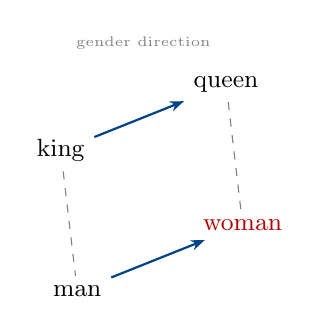
\begin{tikzpicture}[scale=1.05,
  every node/.style={font=\small},
  arr/.style={-{Stealth[length=5pt]}, thick, color=unibo}]

  \node (king)  at (0.0, 2.2) {king};
  \node (queen) at (2.0, 3.0) {queen};
  \node (man)   at (0.2, 0.5) {man};
  \node (woman) at (2.2, 1.3) {\textcolor{red!70!black}{woman}};

  \draw[arr] (king)  -- (queen);
  \draw[arr] (man)   -- (woman);

  \draw[dashed, gray, thin] (king) -- (man);
  \draw[dashed, gray, thin] (queen) -- (woman);

  \node[gray, font=\tiny] at (1.0, 3.5) {gender direction};
\end{tikzpicture}

\medskip
\small
Parallel arrows indicate that the vector offset encoding a relationship
is \emph{consistent} across different word pairs.

\end{columns}

\end{frame}
%
%..................................................................
%
\begin{frame}{Critical Assessment: What This Notebook Does and Does Not Show}

\begin{block}{What the notebook demonstrates effectively}
  \begin{itemize}
    \item Analogy accuracy is a reproducible and interpretable metric for
          comparing embedding corpora.
    \item Training corpus quality and domain coverage dominate corpus size.
    \item Geometric linearity of semantic relationships is real and
          visually verifiable in the 2D projection.
  \end{itemize}
\end{block}
\end{frame}
%
%..................................................................
%
\begin{frame}{Critical Assessment: What This Notebook Does and Does Not Show}
\begin{alertblock}{What the notebook does not tell us}
  \begin{itemize}
    \item \textbf{Analogy accuracy $\neq$ downstream task performance.}
          High analogy scores do not guarantee good sentiment
          classification, NER, or sequence modelling.
    \item \textbf{Currency and finance-domain analogies fail.}
          The benchmark confirms the domain gap rather than resolving it.
    \item \textbf{The 2D visualisation is highly lossy.}
          Apparent non-parallelism in plots may reflect projection
          artefacts, not true embedding failures.
    \item \textbf{Static embeddings cannot handle polysemy.}
          A downstream task on central bank communications would
          need contextual representations (BERT, FinBERT) to correctly
          distinguish, for instance, the monetary and physical senses
          of ``tightening''.
  \end{itemize}
\end{alertblock}

\end{frame}
%
%..................................................................
%
\begin{frame}{Summary}

\begin{columns}[T]
\column{0.5\textwidth}
\textbf{Four-step workflow}
\begin{enumerate}
  \item Convert GloVe $\to$ word2vec format
        (add vocabulary/dimension header)
  \item Inspect file structure before loading
        (validate header, count lines, flag bad tokens)
  \item Evaluate on word analogy benchmark
        across Twitter, Wikipedia, Common Crawl
  \item Visualise geometry via PCA projection
        and displacement parallelism plots
\end{enumerate}

\column{0.5\textwidth}
\textbf{Key takeaways}
\begin{itemize}
  \item Wikipedia and Common Crawl vectors
        substantially outperform Twitter vectors.
  \item Currency analogies fail everywhere —
        a direct consequence of domain mismatch.
  \item Analogy evaluation is a useful but
        incomplete proxy for downstream utility.
  \item Static embeddings are the natural
        starting point for understanding dense
        representations; their limitations
        motivate contextual models covered
        in Lesson~3.
\end{itemize}
\end{columns}

\bigskip
\begin{center}
  \small
  \textit{Notebook Reference:} Jansen (2020), \emph{ML for Algorithmic Trading},
  Chapter 16 on Word Embeddings
\end{center}
\end{frame}
%__________________________________________________________________________
%
\begin{frame}[plain]
\centering
\vspace{1.0cm}
\LARGE{\textbf{Section 2}}
\vspace{0.5cm}

{\Huge \textbf{Financial News Pre-Processing}}

\vspace{1.5cm}

{\large
\begin{tabular}{@{}l l@{}}
\textbf{Notebooks:} 
& \texttt{03\_financial\_news\_preprocessing} \\[0.3em]
& \texttt{ }
\end{tabular}
}

\end{frame}
%__________________________________________________________________________
%
\begin{frame}{Motivation \& Context}

  \begin{columns}[T]
    \begin{column}{0.55\textwidth}
      \begin{block}{Why preprocess financial news?}
        \begin{itemize}
          \item Word embedding models (Word2Vec, GloVe) require
                \textbf{clean, tokenised, lower-cased} text.
          \item Raw news feeds contain HTML entities, numbers,
                punctuation and boilerplate that \alert{corrupt
                the embedding space}.
          \item Financial language is domain-specific:
                multi-word expressions such as
                \textit{central\_bank} or \textit{interest\_rate}
                carry atomic meaning and must be preserved
                as \textbf{n-grams}.
        \end{itemize}
      \end{block}
    \end{column}
    \begin{column}{0.42\textwidth}
      \begin{block}{Data source}
        \begin{itemize}
          \item \textbf{US Financial News} dataset
                (JSON archive)
          \item Sources: CNBC, Reuters (Business, World,
                Technology, Money), WSJ
          \item Each article stored as a JSON object
                with \texttt{thread.section\_title}
                and \texttt{text} fields
        \end{itemize}
      \end{block}
    \end{column}
  \end{columns}

\end{frame}
%
%..................................................................
%
\begin{frame}{End-to-End Preprocessing Pipeline}

\begin{center}
\resizebox{0.98\textwidth}{!}{%
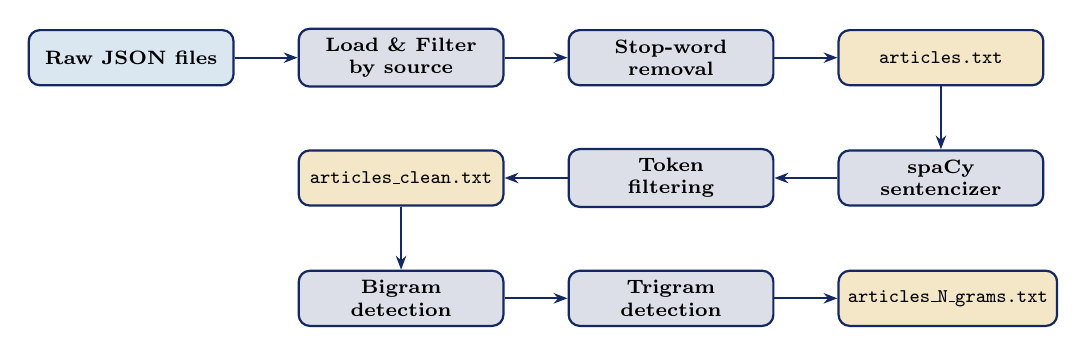
\begin{tikzpicture}[
    node distance = 0.55cm and 0.8cm,
    box/.style    = {rectangle, rounded corners=4pt,
                     minimum width=2.6cm, minimum height=0.7cm,
                     align=center,
                     font=\scriptsize\bfseries,
                     draw=NavyBlue, line width=0.8pt},
    inp/.style    = {box, fill=SteelBlue!20},
    proc/.style   = {box, fill=NavyBlue!15},
    outbox/.style = {box, fill=AccentGold!25},
    arr/.style    = {-{Stealth[length=5pt]}, thick, color=NavyBlue},
  ]

  \node[inp]  (raw)    {Raw JSON files};
  \node[proc, right=of raw]   (load)   {Load \& Filter\\by source};
  \node[proc, right=of load]  (stop)   {Stop-word\\removal};
  \node[outbox,  right=of stop]  (art)    {\texttt{articles.txt}};

  \node[proc, below=0.8cm of art]   (spacy)  {spaCy\\sentencizer};
  \node[proc, left=of spacy]  (clean)  {Token\\filtering};
  \node[outbox,  left=of clean]  (cart)   {\texttt{articles\_clean.txt}};

  \node[proc, below=0.8cm of cart]  (bigram) {Bigram\\detection};
  \node[proc, right=of bigram](trigram){Trigram\\detection};
  \node[outbox,  right=of trigram](ngout) {\texttt{articles\_N\_grams.txt}};

  \draw[arr] (raw)    -- (load);
  \draw[arr] (load)   -- (stop);
  \draw[arr] (stop)   -- (art);
  \draw[arr] (art)    -- (spacy);
  \draw[arr] (spacy)  -- (clean);
  \draw[arr] (clean)  -- (cart);
  \draw[arr] (cart)   -- (bigram);
  \draw[arr] (bigram) -- (trigram);
  \draw[arr] (trigram)-- (ngout);

\end{tikzpicture}%
}
\end{center}

\vspace{0.3em}

\begin{columns}[T]
  \begin{column}{0.32\textwidth}
    \centering\footnotesize
    \textbf{Stage 1 \textemdash{} Ingest}\\
    JSON parsing, source filtering, initial stop-word stripping
  \end{column}

  \begin{column}{0.32\textwidth}
    \centering\footnotesize
    \textbf{Stage 2 \textemdash{} Clean}\\
    Sentence segmentation, token-level quality filtering
  \end{column}

  \begin{column}{0.32\textwidth}
    \centering\footnotesize
    \textbf{Stage 3 \textemdash{} N-grams}\\
    Statistical collocation detection (Gensim Phrases)
  \end{column}
\end{columns}

\end{frame}
%
%..................................................................
%
\begin{frame}[fragile]{Stage 1 — Data Ingestion \& Source Filtering}

  \begin{columns}[T]
    \begin{column}{0.52\textwidth}
      \begin{block}{Trusted section titles (11 sources)}
        \begin{itemize}
          \item Press Releases — CNBC
          \item Reuters: Company / World / Business News
          \item Reuters: Financial Services \& Real Estate
          \item Reuters: Money / Technology News
          \item Top News and Analysis (pro)
          \item The Wall Street Journal — Breaking News
        \end{itemize}
      \end{block}
      \vspace{0.3em}
      \begin{block}{Stop-word list}
        \scriptsize
        Downloaded from the Glasgow IR Resources server
        (\textasciitilde571 common English words).
        Applied at \textbf{word-token level} before saving to
        \texttt{articles.txt}.
      \end{block}
    \end{column}
    \begin{column}{0.46\textwidth}
    \scriptsize
\begin{lstlisting}
def read_articles():
 articles, counter = [], Counter()
 for f in data_path.glob('*/**/*.json'):
   with f.open("r", encoding="utf-8") 
              as fp:
     article = json.load(fp)
   if article['thread']['section_title']
             in set(section_titles):
      text = article['text'].lower()
                            .split()
      counter.update(text)
      articles.append(
         ' '.join([t for t in text
         if t not in stop_words])
      )
    return articles, counter
\end{lstlisting}
      \vspace{0.2em}
      \alert{\scriptsize Note:} explicit \texttt{utf-8} encoding prevents
      Windows \texttt{cp1252} errors.
    \end{column}
  \end{columns}

\end{frame}
%
%..................................................................
%
\begin{frame}[fragile]{Stage 2 — Sentence Segmentation \& Token Filtering}
\small
  \begin{columns}[T]
    \begin{column}{0.50\textwidth}
      %\vspace{-.5cm}
      \begin{block}{spaCy pipeline}
        \begin{itemize}
          \item Blank English model (\texttt{spacy.blank("en")})
          \item \textbf{Sentencizer} component added:
                rule-based, fast, no POS/NER overhead
          \item Batched inference via \texttt{nlp.pipe}
                (\texttt{batch\_size=100},
                 \texttt{n\_process=8})
        \end{itemize}
      \end{block}
      \begin{block}{Sentence quality gates}
        A sentence is \textbf{kept} if and only if:
        \begin{itemize}
          \item $\geq 6$ valid tokens after filtering
          \item $< 100$ raw spaCy tokens (removes
                boilerplate ``mega-sentences'')
        \end{itemize}
      \end{block}
    \end{column}
    \begin{column}{0.48\textwidth}
    \vspace{-.3cm}
\begin{lstlisting}
def clean_doc(d):
    doc = []
    for sent in d.sents:
        s = [
            t.text.lower()
            for t in sent
            if not any([
                t.is_digit,
                not t.is_alpha,
                t.is_punct,
                t.is_space
            ])
        ]
        if len(s) > 5 and 
           len(sent) < 100:
            doc.append(' '.join(s))
    return doc
\end{lstlisting}
      %\vspace{0.2em}
      %\begin{alertblock}{\scriptsize Token filter logic}
      %  \scriptsize Keep only tokens that are \textbf{alphabetic},
      %  non-digit, non-punctuation and non-whitespace.
      %  Lowercased before appending.
      %\end{alertblock}
    \end{column}
  \end{columns}

\end{frame}
%
%..................................................................
%
\begin{frame}{Corpus Statistics}
\small
  \begin{columns}[T]
    \begin{column}{0.50\textwidth}
      \begin{block}{What is measured}
        After writing \texttt{articles\_clean.txt}, the notebook
        computes:
        \begin{itemize}
          \item \textbf{Vocabulary size}: unique tokens
                (further filtered against stop-words)
          \item \textbf{Sentence-length distribution}:
                \texttt{pd.Series.describe} with decile
                percentiles (\texttt{np.arange(.1, 1, .1)})
          \item \textbf{Top-25 tokens}: horizontal bar chart
                (most frequent non-stop-word types)
        \end{itemize}
      \end{block}
      \vspace{0.4em}
      %\begin{alertblock}{Diagnostic purpose}
      %  These statistics confirm that cleaning did not
      %  under-/over-strip the corpus before feeding
      %  it to Gensim.
      %\end{alertblock}
    \end{column}
    \begin{column}{0.46\textwidth}
      \begin{block}{Key metrics (illustrative)}
        \begin{tabular}{lc}
          \toprule
          Metric & Value \\
          \midrule
          Sentences (raw)        & $N$ articles \\
          Sentences (clean)      & $< N$ (quality filter) \\
          Median sentence length & $\sim$12 tokens \\
          Vocabulary (filtered)  & $\sim$tens of thousands \\
          \bottomrule
        \end{tabular}
        \vspace{0.4em}

        \scriptsize Exact counts depend on the corpus snapshot.
        The notebook prints live counts at runtime.
      \end{block}
      %\vspace{0.3em}
      %\begin{block}{Visualisation}
      %  \scriptsize Horizontal bar chart of the 25 most common
      %  tokens (Seaborn / Matplotlib, \texttt{figsize=(14,6)}).
      %  Used to validate domain relevance of vocabulary.
      %\end{block}
    \end{column}
  \end{columns}

\end{frame}
%
%..................................................................
%
\begin{frame}[fragile]{Stage 3 — Statistical N-Gram Detection}
  \begin{columns}[T]
    \begin{column}{0.45\textwidth}
      \begin{block}{Gensim \texttt{Phrases} / \texttt{Phraser}}
        \begin{itemize}
          \item \textbf{Iterative}: bigrams first, then
                trigrams built on top of bigrams
          \item \textbf{Scoring hyper-parameters}:
                \texttt{threshold=100},
                \texttt{min\_count=10}
          \item A phrase $(w_i, w_{i+1})$ is promoted when
                its collocation score exceeds the threshold
          \item Joined with underscore:
                \texttt{interest\_rate},
                \texttt{central\_bank}
        \end{itemize}
      \end{block}
    \end{column}
    \begin{column}{0.55\textwidth}
\scriptsize
\begin{lstlisting}
sentences = LineSentence(clean_article_path)

for n in range(2, max_length + 1):   # 2, 3
    if n > 2:
        sentences = LineSentence(
            results_path /
            f'articles_{n-1}_grams.txt'
        )
    phrases = Phrases(sentences,
                      threshold=100,
                      min_count=10)
    phrase_scores = phrases
                    .find_phrases(sentences)
    grams = Phraser(phrases)
    sentences = grams[sentences]
    with open(f'articles_{n}_grams.txt','w') 
             as f:
        for sent in sentences:
            f.write(' '.join(sent) + '\n')
\end{lstlisting}
      %\vspace{0.2em}
      %\alert{\scriptsize Note:} \texttt{find\_phrases()} returns a
      %\texttt{dict\{phrase: score\}};
      %converted to a ranked \texttt{DataFrame} for inspection.
    \end{column}
  \end{columns}

\end{frame}
%
%..................................................................
%
\begin{frame}{Key Libraries \& Design Choices}
\small
  \begin{columns}[T]
    \begin{column}{0.48\textwidth}
      \begin{block}{Library stack}
        \begin{tabular}{ll}
          \toprule
          Library & Role \\
          \midrule
          \textbf{spaCy}   & Sentence segmentation \\
          \textbf{Gensim}  & Phrase detection \& corpus I/O \\
          \textbf{pandas}  & Stats \& top-token ranking \\
          \textbf{Seaborn} & Frequency visualisation \\
          \textbf{pathlib} & Cross-platform path handling \\
          \bottomrule
        \end{tabular}
      \end{block}
      \begin{block}{Reproducibility}
        \begin{itemize}
          \item \texttt{np.random.seed(42)} set globally
          \item All file I/O uses explicit \texttt{utf-8}
                encoding
        \end{itemize}
      \end{block}
    \end{column}
    \begin{column}{0.48\textwidth}
      \begin{block}{Design decisions}
        \begin{itemize}
          \item \textbf{Blank spaCy model}: avoids loading
                the full statistical pipeline (POS, NER)
                which is unnecessary for sentence splitting
                — significantly faster on large corpora
          \item \textbf{LineSentence}: memory-efficient
                streaming from disk; no need to load the
                full corpus into RAM
          %\item \textbf{Phraser} (frozen model): faster
          %      scoring than live \texttt{Phrases} object
          %      during corpus transformation
          \item \textbf{Two-pass n-gram building}: ensures
                trigrams subsume coherent bigrams, giving
                semantically richer compound tokens
        \end{itemize}
      \end{block}
    \end{column}
  \end{columns}

\end{frame}
%
%..................................................................
%
\begin{frame}{Summary}
\small
  \begin{columns}[T]
    \begin{column}{0.55\textwidth}
      \begin{block}{What this notebook delivers}
        \begin{enumerate}
          \item \textbf{Filtered corpus}: only articles from
                trusted financial news sections (CNBC,
                Reuters, WSJ)
          \item \textbf{Clean sentence corpus}:
                lower-cased, alphabetic-only tokens,
                quality-gated sentences
          \item \textbf{N-gram corpus} (up to trigrams):
                domain-relevant collocations preserved
                as atomic units
          \item \textbf{Corpus statistics}: vocabulary size,
                sentence-length distribution, top-token
                frequency chart
        \end{enumerate}
      \end{block}
    \end{column}
    \begin{column}{0.42\textwidth}
      \begin{alertblock}{Downstream use}
        The file \texttt{articles\_3\_grams.txt} is the
        direct input to \textbf{Word2Vec training},
        enabling the model to learn embeddings that
        capture financial collocations as single vectors.
      \end{alertblock}
      \vspace{0.4em}
      \begin{block}{Artefacts produced}
        \scriptsize
        \begin{tabular}{ll}
          \texttt{articles.txt}          & Raw (stop-word filt.) \\
          \texttt{articles\_clean.txt}   & Sentence-cleaned \\
          \texttt{articles\_2\_grams.txt}& Bigram corpus \\
          \texttt{articles\_3\_grams.txt}& Trigram corpus \\
        \end{tabular}
      \end{block}
    \end{column}
  \end{columns}

  \vspace{0.5em}
  \begin{center}
    \small\textit{``Good embeddings start with good text cleaning.''}
  \end{center}

\end{frame}
%__________________________________________________________________________
%
\begin{frame}[plain]
\centering
\vspace{1.0cm}
\LARGE{\textbf{Section 3}}
\vspace{0.5cm}

{\Huge \textbf{Training Word2Vec on Financial News}}

\vspace{1.5cm}

{\large
\begin{tabular}{@{}l l@{}}
\textbf{Notebooks:} 
& \texttt{04\_financial\_news\_word2vec\_tensorflow.ipynb} \\[0.3em]
& \texttt{05\_financial\_news\_word2vec\_gensim.ipynb}
\end{tabular}
}

\end{frame}
%__________________________________________________________________________
%
\begin{frame}{Why Train Custom Financial Embeddings?}

  \begin{itemize}
    \setlength\itemsep{0.7em}
    \item Generic pre-trained models (GloVe, Word2Vec/Wikipedia) \textbf{miss
          financial vocabulary}: \textit{quantitative easing},
          \textit{yield\_curve}, \textit{earnings\_guidance}, \ldots
    \item Domain language \textbf{shifts over time} — new products,
          regulations and crises continuously introduce unseen words.
    \item Out-of-vocabulary words receive a \alert{default zero-information
          vector}, degrading all downstream tasks.
    \item Corporate earnings releases and Reuters wire stories use
          \textbf{nuanced co-occurrence patterns} that general corpora
          do not capture.
  \end{itemize}

  \vspace{0.8em}
  \begin{alertblock}{Solution}
    Train Word2Vec \textbf{from scratch} on the preprocessed financial
    news corpus produced by Notebook 03.
  \end{alertblock}

\end{frame}
%
%..................................................................
%
\begin{frame}{Shared Setup Across Both Notebooks}

  \begin{columns}[T]
    \begin{column}{0.48\textwidth}
      \begin{block}{Common inputs}
        \begin{itemize}
          \item Corpus: \texttt{articles\_3\_grams.txt}
                (output of NB\,03)
          \item Algorithm: \textbf{Word2Vec Skip-gram}
          \item Evaluation: Google word-analogy benchmark
                (\texttt{analogies-en.txt})
        \end{itemize}
      \end{block}
    \end{column}
    \begin{column}{0.48\textwidth}
      \begin{block}{Common hyperparameters}
        \begin{tabular}{|l|l|}
          \hline
          \textbf{Parameter} & \textbf{Value} \\
          \hline
          Embedding dimension & 300 \\
          N-gram order        & 3 (trigrams) \\
          Loss                & Negative Sampling \\
          \hline
        \end{tabular}
      \end{block}
    \end{column}
  \end{columns}

  \vspace{0.8em}
  \begin{block}{Two complementary perspectives}
    \begin{itemize}
      \item \textbf{NB\,04 (Keras/TF)}: builds Word2Vec \emph{from scratch}
            to expose every architectural detail.
      \item \textbf{NB\,05 (Gensim)}: uses an optimised C-level backend
            for fast, production-grade training.
    \end{itemize}
  \end{block}

\end{frame}
%
%..................................................................
%
\begin{frame}{The Skip-Gram Model}

  \begin{block}{Core objective}
    Given target word $w_t$, predict surrounding context within window $k$:
    \[
      \max \sum_{-k \le j \le k,\; j \ne 0} \log P(w_{t+j} \mid w_t)
    \]
  \end{block}

  \vspace{0.4em}
  \begin{columns}[T]
    \begin{column}{0.48\textwidth}
      \begin{block}{Negative Sampling}
        Replaces softmax $\mathcal{O}(V)$ with a binary classifier
        that distinguishes \textbf{real pairs} from
        \textbf{noise pairs} — cost drops to
        $\mathcal{O}(k_{\text{neg}})$.
      \end{block}
    \end{column}
    \begin{column}{0.48\textwidth}
      \begin{block}{Subsampling}
        Frequent words downsampled with
        $P(w) = 1 - \sqrt{t / f(w)}$,
        balancing rare and common tokens.
      \end{block}
    \end{column}
  \end{columns}
\end{frame}
%
%..................................................................
%
\begin{frame}[fragile]{NB\,04 — Keras: Data Preparation}

  \begin{columns}[T]
    \begin{column}{0.44\textwidth}
      \begin{block}{Token-to-ID mapping}
        \begin{enumerate}\small
          \item Keep tokens with \texttt{MIN\_FREQ} $\ge 10$
          \item Assign integer IDs; unknown $\to 0$
          \item Drop sentences $> 50$ tokens
          \item Sample 50\% of sentences
        \end{enumerate}
      \end{block}
      \vspace{0.5em}
      \begin{block}{Pair generation}
        \small
        Keras \texttt{skipgrams()} produces\\
        \texttt{(target, context, label)} triples.\\[0.3em]
        Persisted to \texttt{data.h5} to avoid
        regeneration across runs.
      \end{block}
    \end{column}
    \begin{column}{0.50\textwidth}
\scriptsize
\begin{lstlisting}
# Vocabulary
token_counts = [t for t in
    Counter(words).most_common()
    if t[1] >= MIN_FREQ]
tokens, _ = zip(*token_counts)
id_to_token = dict(enumerate(tokens, 1))
id_to_token[0] = 'UNK'

# Skip-gram pairs
pairs, labels = skipgrams(
    sequence        = data,
    vocabulary_size = vocab_size,
    window_size     = WINDOW_SIZE,
    sampling_table  = sampling_table,
    negative_samples= 1.0,
    shuffle         = True
)
\end{lstlisting}
    \end{column}
  \end{columns}

\end{frame}
%
%..................................................................
%
\begin{frame}[fragile]{NB\,04 — Keras: Model Architecture}

  \begin{columns}[T]
    \begin{column}{0.44\textwidth}
      \begin{block}{Functional Keras graph}
        \begin{enumerate}\small
          \item Two scalar \texttt{Input} layers
          \item \textbf{Shared} \texttt{Embedding}
                ($V \times 300$)
          \item \texttt{Dot} product of the two vectors
          \item \texttt{Dense(1, sigmoid)} output
          \item Loss: \texttt{binary\_crossentropy}\\
                Opt: \texttt{RMSprop}
        \end{enumerate}
      \end{block}
      \vspace{0.4em}
      \begin{alertblock}{\small Validation model}
        \small Same weights, cosine similarity.
        Nearest-neighbour checks and analogy
        accuracy run at each epoch.
      \end{alertblock}
    \end{column}
    \begin{column}{0.50\textwidth}
\scriptsize
\begin{lstlisting}
embedding = Embedding(vocab_size,
    EMBEDDING_SIZE, input_length=1)

target  = Reshape((EMBEDDING_SIZE, 1))(
              embedding(input_target))
context = Reshape((EMBEDDING_SIZE, 1))(
              embedding(input_context))

dot = Dot(axes=1)([target, context])
out = Dense(1, activation='sigmoid')(dot)

model = Model(
    inputs  = [input_target, input_context],
    outputs = out)
model.compile(
    loss      = 'binary_crossentropy',
    optimizer = 'rmsprop')
\end{lstlisting}
    \end{column}
  \end{columns}

\end{frame}
%
%..................................................................
%
\begin{frame}{NB\,04 — Keras: Training \& Visualisation}

  \begin{columns}[T]
    \begin{column}{0.48\textwidth}
      \begin{block}{Training loop}
        \begin{itemize}
          \item \texttt{EPOCHS = 1},
                \texttt{BATCH\_SIZE = 2\,500}
          \item \texttt{EvalCallback} runs at train start,
                epoch end, and train end:
                \begin{itemize}
                  \item Prints $k$-nearest neighbours for
                        10 validation words
                  \item Reports analogy accuracy at
                        top-1, top-5 and top-10
                \end{itemize}
          \item Model saved as \texttt{skipgram\_model.h5}
        \end{itemize}
      \end{block}
    \end{column}
    \begin{column}{0.48\textwidth}
      \begin{block}{TensorBoard integration}
        \begin{itemize}
          \item Token metadata exported to
                \texttt{meta.tsv}
          \item \texttt{TensorBoard} callback writes
                embedding projector logs
          \item Enables \textbf{interactive 3-D
                visualisation} of the 300-dimensional
                embedding space directly in the browser
        \end{itemize}
      \end{block}
      \begin{alertblock}{Pedagogical value}
        The explicit Keras graph makes every component
        of Word2Vec directly inspectable and modifiable
        — ideal for understanding the architecture.
      \end{alertblock}
    \end{column}
  \end{columns}

\end{frame}
%
%..................................................................
%
\begin{frame}[fragile]{NB\,05 — Gensim: Model Training}

  \begin{columns}[T]
    \begin{column}{0.48\textwidth}
      \begin{block}{Single-call training}
        The entire pipeline — vocabulary building,
        subsampling, negative sampling, multi-threaded
        SGD — is wrapped in one constructor:
      \end{block}
\scriptsize
\begin{lstlisting}
model = Word2Vec(
    sentences = LineSentence(sentence_path),
    sg         = 1,     # Skip-gram
    vector_size= 300,
    window     = 5,
    min_count  = 100,
    negative   = 20,
    workers    = 8,
    epochs     = 1,
    alpha      = 0.05
)
\end{lstlisting}
    \end{column}
    \begin{column}{0.48\textwidth}
      \begin{block}{Key differences vs NB\,04}
        \begin{itemize}
          \item \texttt{min\_count = 100} (vs 10 in NB\,04)
                — keeps only well-attested words
          \item \texttt{negative = 20} noise samples
                (vs 1) — much stronger gradient signal
          \item \texttt{window = 5} (vs 3)
          \item \texttt{workers = 8} — true
                multi-threaded C backend
          \item \texttt{LineSentence} streams from disk
                — no full corpus loaded into RAM
        \end{itemize}
      \end{block}
    \end{column}
  \end{columns}

\end{frame}
%
%..................................................................
%
\begin{frame}[fragile]{NB\,05 — Gensim: Incremental Training \& Checkpointing}

  \begin{columns}[T]
    \begin{column}{0.50\textwidth}
      \begin{block}{Training loop (up to 10 epochs)}
        After the initial epoch, the model is trained
        for up to 9 additional epochs via
        \texttt{model.train()}.\\[0.4em]
        After each epoch:
        \begin{itemize}
          \item Analogy accuracy is evaluated with
                \texttt{evaluate\_word\_analogies()}
          \item Model is \textbf{checkpointed only when
                accuracy improves} (best-model tracking)
          \item Accuracy history saved to
                \texttt{accuracies.csv}
        \end{itemize}
      \end{block}
    \end{column}
    \begin{column}{0.48\textwidth}
\scriptsize
\begin{lstlisting}
for i in range(1, 10):
    model.train(
        sentences,
        epochs=1,
        total_examples=model.corpus_count
    )
    score, details = model.wv\
        .evaluate_word_analogies(
            analogy_path,
            case_insensitive=True
        )
    if score > best_accuracy:
        model.save(f"word2vec_{i}.model")
        model.wv.save(
            f"word_vectors_{i}.kv")
        best_accuracy = score
\end{lstlisting}
    \end{column}
  \end{columns}

\end{frame}
%
%..................................................................
%
\begin{frame}{NB\,05 — Gensim: Evaluation}

  \begin{columns}[T]
    \begin{column}{0.48\textwidth}
      \begin{block}{Analogy benchmark — 14 categories}
        \begin{itemize}
          \item \textit{Semantic}: capitals, currencies,
                family relations, city-state pairs
          \item \textit{Syntactic}: comparatives,
                superlatives, past tense, plurals,
                present participle, \ldots
        \end{itemize}
        Results shown per category as a stacked bar chart
        (correct vs incorrect) with accuracy overlay.
      \end{block}
    \end{column}
    \begin{column}{0.48\textwidth}
      \begin{block}{Qualitative checks}
        \begin{itemize}
          \item \textbf{Classic analogy}: \\
                \textit{king} $-$ \textit{man}
                $+$ \textit{woman} $\approx$ \textit{queen}
          \item \textbf{Most-similar lookup}: for 10
                randomly sampled frequent tokens, print
                the 10 nearest neighbours in cosine space
          \item Results exported to
                \texttt{most\_similar.csv}
        \end{itemize}
      \end{block}
    \end{column}
  \end{columns}

\end{frame}
%
%..................................................................
%
\begin{frame}{NB\,04 vs NB\,05 — Side-by-Side Comparison}

\begin{columns}[T]
  \begin{column}{0.48\textwidth}
    \begin{block}{NB\,04 — Keras / TensorFlow}
      \begin{itemize}\small
        \item \textbf{Purpose:} expose architecture step by step
        \item \textbf{Pairs:} manual via \texttt{skipgrams()}
        \item \textbf{Negatives:} 1 sample
        \item \textbf{Epochs:} fixed at 1
        \item \textbf{Speed:} slower — Python-level TF graph
        \item \textbf{Viz:} TensorBoard 3-D projector
        \item \textbf{Output:} \texttt{skipgram\_model.h5}
      \end{itemize}
    \end{block}
  \end{column}
  \begin{column}{0.48\textwidth}
    \begin{block}{NB\,05 — Gensim}
      \begin{itemize}\small
        \item \textbf{Purpose:} fast, production-grade training
        \item \textbf{Pairs:} handled internally by Gensim
        \item \textbf{Negatives:} 20 samples
        \item \textbf{Epochs:} up to 10, accuracy checkpointing
        \item \textbf{Speed:} faster — multi-threaded C backend
        \item \textbf{Viz:} Matplotlib bar charts + CSV
        \item \textbf{Output:} \texttt{word2vec.model} + \texttt{.kv}
      \end{itemize}
    \end{block}
  \end{column}
\end{columns}

\vspace{0.5em}
\begin{alertblock}{}
  \centering\small
  Same algorithm, same goal — Keras reveals \textit{how} it works;
  Gensim reveals \textit{how well} it can be trained at scale.
\end{alertblock}

\end{frame}
%
%..................................................................
%
\begin{frame}{Key Takeaways}

  \begin{enumerate}
    \setlength\itemsep{0.7em}
    \item \textbf{Domain specificity matters.}
          Training on financial news produces embeddings that correctly
          cluster \textit{yield}, \textit{rate}, \textit{bond} and
          related terms — not possible with generic GloVe vectors.

    \item \textbf{N-grams add value.}
          Trigram pre-processing (NB\,03) ensures that
          \textit{central\_bank} and \textit{interest\_rate}
          are treated as single atomic tokens.

    \item \textbf{Keras = transparency; Gensim = performance.}
          Use NB\,04 to understand the model;
          use NB\,05 to train it seriously.

    \item \textbf{Analogy accuracy as a relative signal.}
          The benchmark is imperfect for financial text,
          but provides a consistent metric to compare
          configurations and select the best epoch checkpoint.
  \end{enumerate}

\end{frame}
%
%===================================================================================================
%
\end{document}
%
%===================================================================================================
%
